In this section the concept of heuristic is explored in some of algorithms used to solve the TSP problem. In particular a set of methods will be presented such as greedy algorithm, extra mileage, and 2-opt optimization.

\subsection{Greedy algorithm}
\label{sec:greedy}
This type of method is the easiest to understand and implement. This heuristic has its base on the concept to construct the shortest path by connecting the nearest nodes.

This algorithm starts from an arbitrary node and chooses its following node by selecting the nearest one from the ones that are not already in the path. This greedy approach is also called Nearest Neighbor.

The main side effect it has is that the shortest path is easily missed since the last nodes - apart from special cases - are far from each other. In this way, the optimal solution is surely not selected. The algorithm is the following: 

\begin{algorithm}
	\caption{Greedy}\label{algo:greedy}
	\begin{algorithmic}[1]
		\Require $G=(V,E)$,$ c:E\rightarrow \Re^+$
		\Ensure $z\text{ hopefully good solution}$
		\State $best\_cost$ $\gets$ $+\infty$
		\State $z$ $\gets$ *empty*
		
		\For{$start\_node$ $\gets$1 $to$ n}
			\State $current\_node$ $\gets$ $start\_node$
			\While{*each node is visited*}
			\State $candidate\_node \gets$ $-1$
				\For{$i \gets 1$ $to$ n}
					\State *Finds the nearest node and marks it as visited*
					\State $candidate\_node \gets$ *nearest node*
				\EndFor
				\State *Saves $candidate\_node$ as next node*
				\State $current\_node$ $\gets$ $candidate\_node$
			\EndWhile
			\If{cost($z_{curr}$)$<best\_cost$}
				\State $best\_cost$ $\gets$ $cost(z_{curr})$
				\State $z$ $\gets$ $z_{curr}$
			\EndIf
		\EndFor
		\State \Return $z$
	\end{algorithmic}
\end{algorithm}

This algorithm describes exactly the behavior of the greedy algorithm. In my implementation, each node is tested as starting node to obtain the best nearest neighbor solution. The classic implementation has a complexity of $O(n^2)$ since each node has to search the nearest node all over the graph. In particular \ref{algo:greedy} has a complexity of $O(n^3)$ because of the aforementioned method to select the best starting node.\\
This complexity is quite low but with some instances with a great number of nodes can be slower than expected.

\subsection{Extra mileage approach}
\label{sec:extra-mileage}
This approach is more complex than the previous one but in favor of a better solution. The main idea behind this algorithm is very simple and it starts from an empty solution and provides a good solution.

It starts with connecting with a cycle the farthest nodes in the instance, this will be the beginning of the solution. Then the closest node among the active edges is selected and is added to the solution. This action is performed by replacing the edge with two more that allow the new node to enter the solution.

\begin{figure}
	\centering
	\begin{subfigure}[b]{0.3\textwidth}
		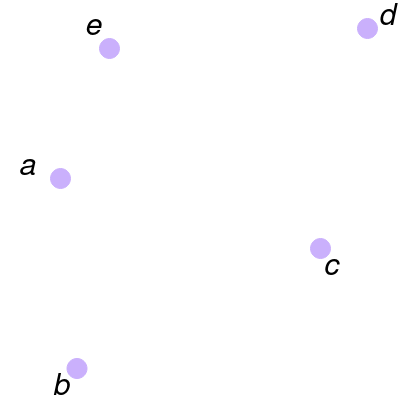
\includegraphics[width=\textwidth]{images/extra_1}
		\caption{No edges}
	\end{subfigure}
	\hfill
	\begin{subfigure}[b]{0.3\textwidth}
		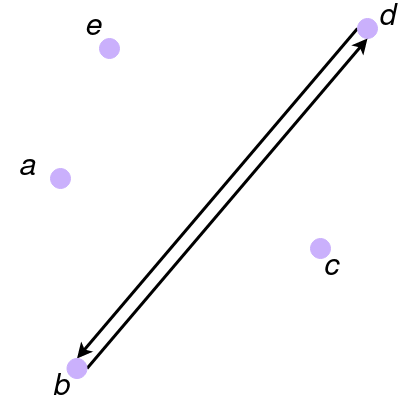
\includegraphics[width=\textwidth]{images/extra_2}
		\caption{First two edges added}
	\end{subfigure}
	\hfill
	\begin{subfigure}[b]{0.3\textwidth}
		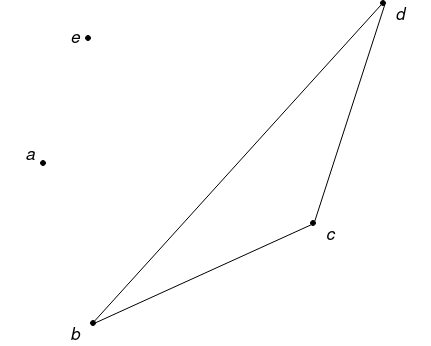
\includegraphics[width=\textwidth]{images/extra_3}
		\caption{One edge is substituted with other two connecting one more node}
	\end{subfigure}
	\bigskip
	\begin{subfigure}{0.3\textwidth}
		\centering
		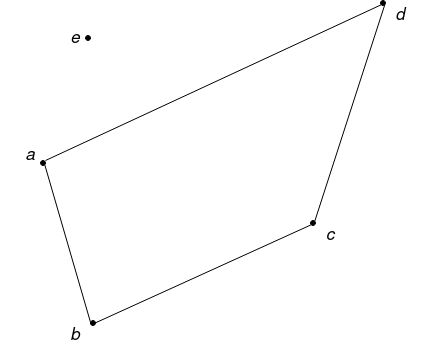
\includegraphics[width=\textwidth]{images/extra_4}
		\caption{Added one more node}
	\end{subfigure}
	\hfill
	\begin{subfigure}{0.3\textwidth}
		\centering
		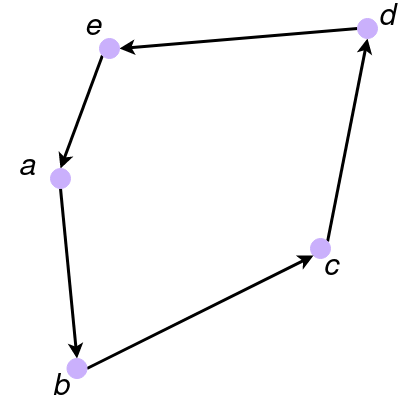
\includegraphics[width=\textwidth]{images/extra_5}
		\caption{All nodes are connected}
	\end{subfigure}
	\caption{In this image we can see the process done by extra-mileage to find the solution.}
	\label{fig:extra}
\end{figure}

The process can be seen in figure \ref{fig:extra} where it is performed with a bunch of nodes.

The method with the next node to be inserted is chosen is the triangle inequality. Actually, with the replacing phase, some cost is added to the solution. Imagine taking into consideration three nodes $(x, y, z)$, where $x$ and $y$ are already in the solution and $z$ wants to join them. The mathematical operation to use is the following:

\begin{equation}
	\Delta(x, y, w) = c_{xw} + c_{yw} - c_{xy}
\end{equation}

This value will always be positive thanks to the aforementioned triangle inequality which states that the sum of the lengths of any two sides must be greater than or equal to the length of the remaining side.

The algorithm used is the following:
\begin{algorithm}
	\caption{Extra mileage}\label{algo:extra-mileage}
	\begin{algorithmic}[1]
		\Require $G=(V,E)$,$ c:E\rightarrow \Re^+$
		\Ensure $z\text{ hopefully good solution}$
		\State $x, y$ $\gets$ *finds the farthest nodes*
		\State $z$ $\gets$ \textsc{Add($x, y$)}
		
		\While{$|z|<n$}
			\State $(x, y, w)$ $\gets$ argmin($\Delta(x, y, w):x, y \in z, w \not \in z$)
			\State $z$ $\gets$ \textsc{Add($w $)}
		\EndWhile
		\State \Return $z$
	\end{algorithmic}
\end{algorithm}

\subsection{2-opt refining}
This section will analyze one refining technique. The target of this approach is to take an existing solution $x$ and try to take it closer to the optimum one.\\
A method to do so is represented by the $k$-opt refining that consists on rearrange $k$ edges in order to obtain a new solution with a lower cost. In particular, this section it is describes the $2$-opt refining.

To apply this approach effectively it is applied starting from a solution obtained with a heuristic approach such as the ones described in section \ref{sec:greedy} and \ref{sec:extra-mileage}. The idea of this algorithm is to remove all the crossing edges and insert new edges that will decrease the cost of the final solution.

To do so it is used the triangle inequality, is used to find the couple of edges that allow the best improvement of the solution. In this implementation the operation is done across four nodes: $i$, $succ[i]$, $j$, and $succ[j]$. Since the tour is asymmetric it has a direction, $succ[i]$ and $succ[j]$ are respectively the following nodes in the path of the nodes $i$ and $j$. 

\begin{equation}
	\label{eqn:2-opt}
	\Delta (i, j) = (c_{i, succ[i]} + c_{j, succ[j]}) - (c_{i, j} + c_{succ[i], succ[j]}) \quad i, j \in V; i\not=succ[j]; j\not=succ[i]
\end{equation}

In \ref{eqn:2-opt} in is described the correct way to compute the delta of the method. Greater the value, better the improving.

\begin{figure}[h]
	\centering
	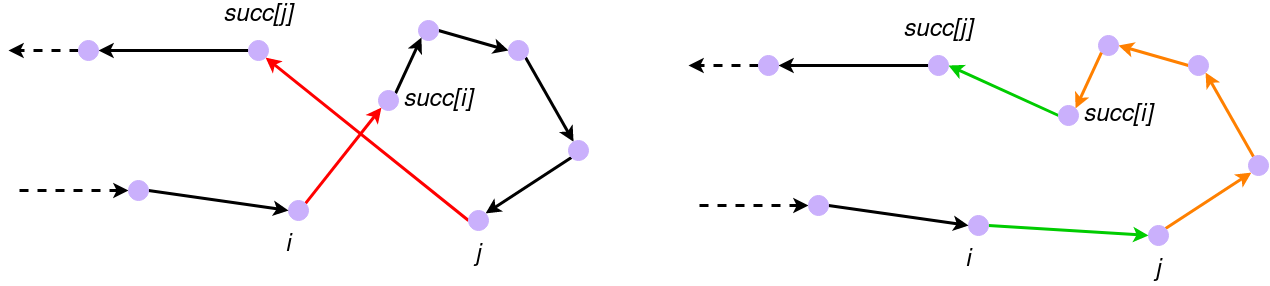
\includegraphics[width=0.9\textwidth]{images/2_opt_new.png}
	\caption{The image represent the replacement of two edges during the $2$-opt refining.}
	\label{fig:2-opt}
\end{figure}

In figure \ref{fig:2-opt} it is possible to notice the replacement of two arcs. A detail to give attention to is that the path from $i$ and $succ[i]$ changes direction after the substitution of the old edges, this is done to maintain the solution integrity. In particular, this optimization is performed until no more $\Delta(i, j)$ positive are found, in that case, the solution is no more improvable by the 2-opt algorithm.

\begin{algorithm}
	\caption{$2$-opt refining}\label{algo:2-opt}
	\begin{algorithmic}[1]
		\Require $G=(V,E)$,$ c:E\rightarrow \Re^+$
		\Ensure $z\text{ hopefully good solution}$
		\State $z$ $\gets$ *find feasible solution with an algorithm*
		\State flag $\gets$ $false$
		
		\While{$flag==false$}
			\State flag $\gets$ $true$
			\State $(i, j)$ $\gets$ argmax($\Delta(i, j):i, j\in V)$
			\If{$\Delta(i, j)>0$}
				\State flag $\gets$ $false$
				\State $z$ $\gets$ *edge replacement*
			\EndIf
		\EndWhile
		\State \Return $z$
	\end{algorithmic}
\end{algorithm}

\begin{figure}
	\centering
	
	\begin{subfigure}[b]{0.45\textwidth}
		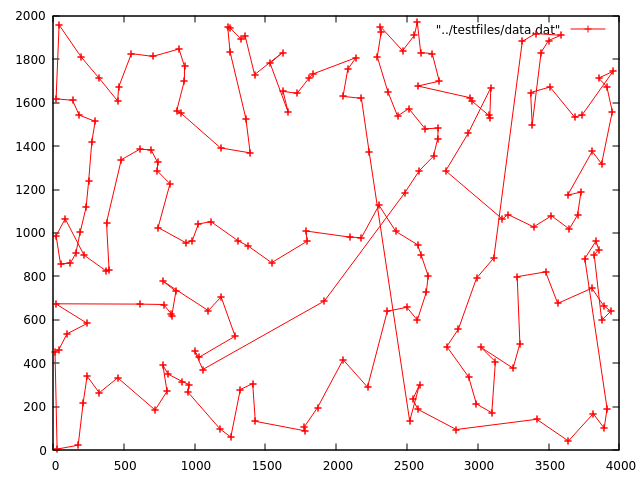
\includegraphics[width=\textwidth]{images/kroA_greedy.png}
	\end{subfigure}
	\hfill
	\begin{subfigure}[b]{0.45\textwidth}
		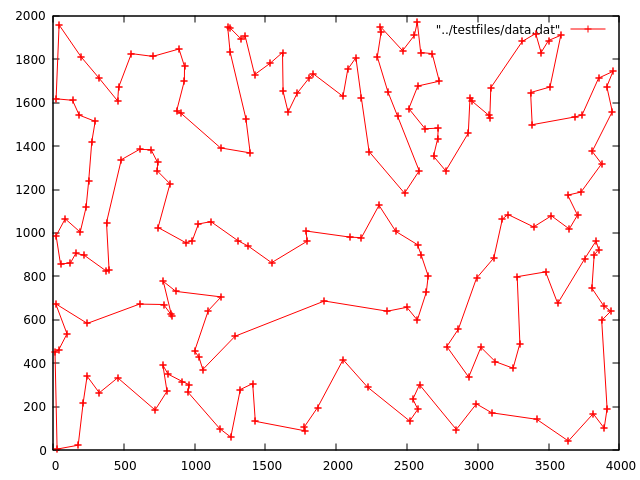
\includegraphics[width=\textwidth]{images/2_opt.png}
	\end{subfigure}
	\caption{The improvement obtained applying to a greedy algorithm (left) the 2-opt refining approach (right).}
\end{figure}